
%%%%%%%%%% Start TeXmacs macros
\newcommand{\nocomma}{}
\newcommand{\noplus}{}
\newcommand{\tmop}[1]{\ensuremath{\operatorname{#1}}}
\newcommand{\tmtextbf}[1]{{\bfseries{#1}}}
\newcommand{\tmtextit}[1]{{#1}}
\newcommand{\tmtexttt}[1]{{\ttfamily{#1}}}
\newenvironment{descriptioncompact}{\begin{description} }{\end{description}}
%%%%%%%%%% End TeXmacs macros


\section{Restricted Boltzmann Machines}

Hopfield networks are deterministc: training a network with the same patterns
will yield the same weights, and matching a pattern against the network will
always give the same result. This has the advantage of simplicity and ease of
testing. However, as mentioned before, there are spirous attractors in the
Hopfields network (liniear combination of an odd number of training patterns).
Using stochastic updating rules will decrease the probability of being 'stuck'
in such a state. This resembles simulated annealing, but ensuring we are not
caught in a local minima (in the energy landscape).

Restricted Boltzmann Machines have been used for various purposes in recent
years (TODO add to bib see
http://uai.sis.pitt.edu/papers/11/p463-louradour.pdf,
http://www.csri.utoronto.ca/\~{ }hinton/absps/nips00-ywt.pdf,
http://www.csri.utoronto.ca/\~{ }hinton/absps/reluICML.pdf), most of it
conducted by Geoffrey E. Hinton at university of Toronto, Canada. They have a
simple structure: one layer of visible units and one layer of hidden units,
which form a bipartite graph, as in Figure. The patterns used to train the
network correspond to the visible (exposed units), while the hidden units
correspond to the attributes of the features we would like to learn. It is
worth mentioning that in the most common and simple form, both the visible and
hidden units take binary values. This is the approach we also adopted for our
implementation.

\ \ \ \ \ \ \ \ \ \ \ \ \ \ \ \ \ \ \ \ \ \ \ \ \ \ \ \ \begin{figure}[h]
  \resizebox{300px}{300px}{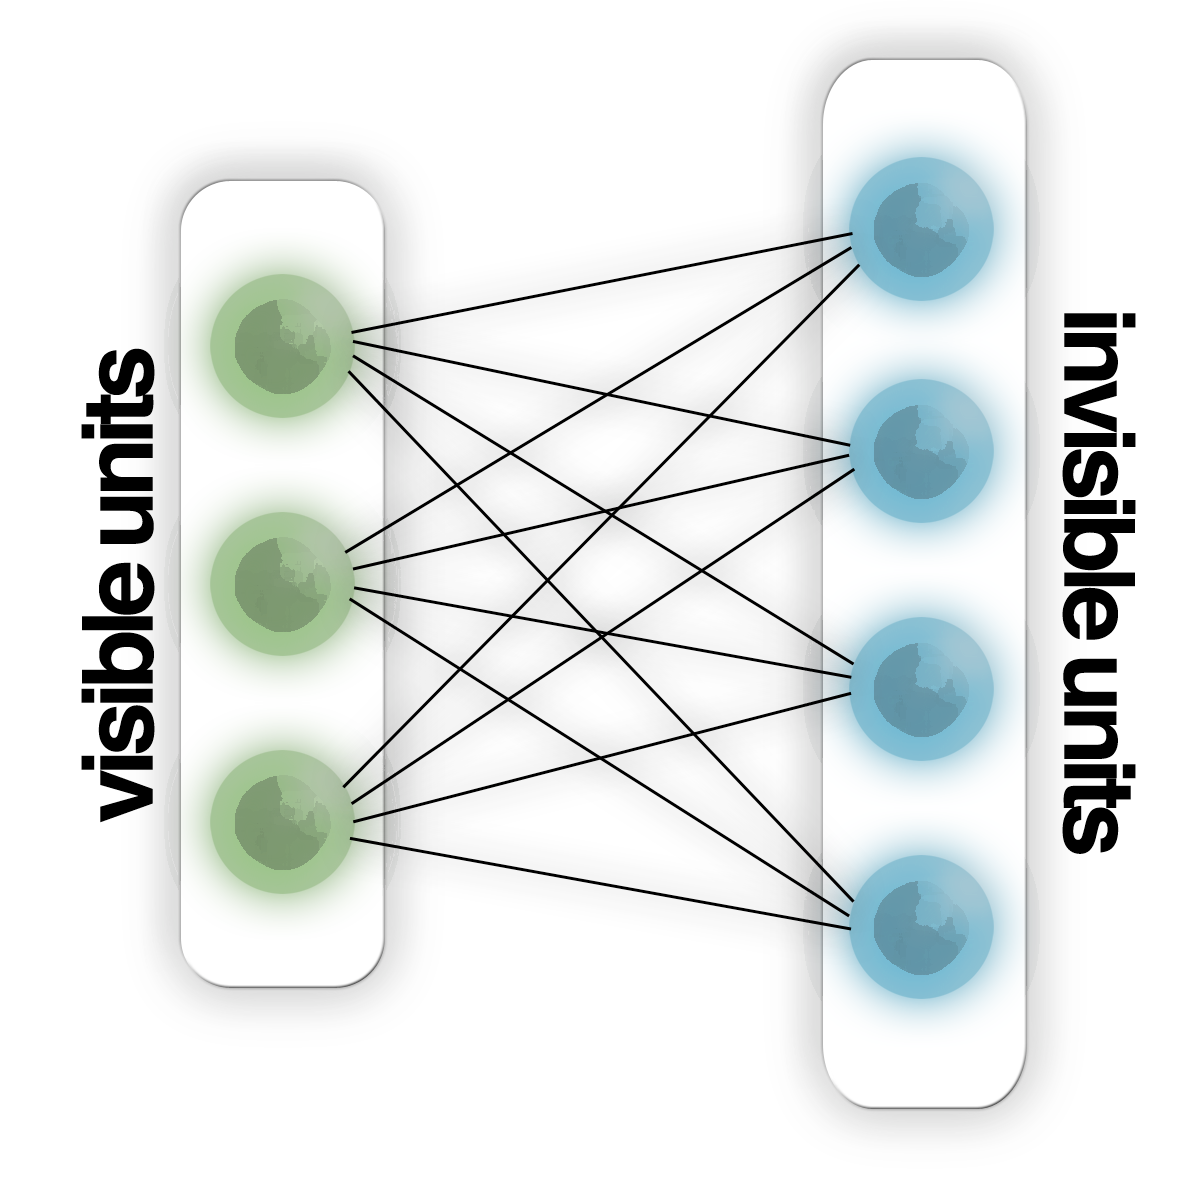
\includegraphics{RBM-1.eps}}
  \caption{Restricted Boltzmann Machine}
\end{figure}


The connections between the neurons in the two layers is symmetrical, so it
can be represented as a weight matrix which keeps the connection beween hidden
and visible layers. A state of a Restricted Boltzmann machins is given by the
values of both the visibile and given state. The corresponding Hopfield energy
formula for a state is given by :
\[ E (v, h) = - \sum_{i \in V} a_i v_i - \sum_{j \in H} b_j h_i - \sum_{i \in
   V, \nocomma j \in H \nocomma} v_i h_j w_{\tmtextit{\tmtextit{\tmop{ij}}}}
\]


where, $w_{\tmtextit{\tmtextit{}}}$is the weight matrix, $a$ and $b$are the
vectors of biases corresponding to the visbile, respectibly hidden layers. As
expected, $v$is vector of visible units and \tmtextit{h} is the vector of
hidden units.

We denote by \tmtextit{V} = \{1, .. \tmtextit{length} \tmtextit{v}\} , the
indices of a visible vector and by \tmtextit{H} = \{1, .. \tmtextit{length}
\tmtextit{h}\} the indices of a hidden vector.



\subsection{Probability of a state}

After traning, the network assigns a probability to each possible state, as
follows:
\[ p \left( v, h \right) = \frac{1}{Z} e^{- E \left( v, h \right)} \]
where Z is used to normalize the probabilities
\[ Z = \sum_{v, h} e^{- E \left( v, h \right)} \]
Thus, the porbability the network assings for a visibile vector \tmtextit{v}:
\begin{equation}
  p \left( v \right) = \sum_h \frac{1}{Z} e^{- E \left( v, h \right)}
\end{equation}

\subsection{Training the network}

The network can be trained such that one maximizes the probabilty of a traning
pattern. The derivative of the log probability of a trainig vector (given by
(1)), is simple, as follows:
\[ \frac{\delta \log p \left( v \right)}{\delta w_{\tmop{ij}}} = < v_i h_i
   >_{\tmop{data}} - < v_i h_i >_{\tmop{model}} \]
Due to the bipartitate nature of the Restricted Boltzmann Machine, it is easy
to attain an \tmtextit{unabiased} sample of the hidden units, given the
visible units.
\begin{equation}
  p \left( h_j = 1 \left|  \right. v \right) = \sigma \left( b_j + \sum_{i \in
  V} v_i w_{\tmop{ij}} \right)
\end{equation}
For the visible units, the same formula gives a \tmtextit{biased} sample of
the visible units.
\begin{equation}
  p \left( v_i = 1 \left|  \right. h \right) = \sigma \left( a_i + \sum_{j \in
  H} h_j w_{\tmop{ij}} \right)
\end{equation}


where $\sigma = \frac{1}{1 \noplus + e^{- x}}^{}$, is the logistic sigmoid
function.

There are ways of getting an unbiased sample of the visible units, but they
are very time consuming. In practice, the contrastive divergence algorithm is
used as a faster substitute. The visibile units are set to a training vector
and the binary states of the hidden vector are computed using (2). These
binary units are used to \tmtextit{reconstruct} the states of the visible
vector using (3).

The training rule then becomes:
\[ \Delta w_{\tmop{ij}} = \lambda \left( < v_i h_i >_{\tmop{data}} - < v_i h_i
   >_{\tmop{reconstruction}} \right) \]
We note that the above training rule has the desired properties for modelling
the biological brain: it is both \tmtextit{local} and \tmtextit{incremental}.
Angle brackets \ denote the expected value under the given distribution by the
following subscript.



\subsection{Using Restricted Boltzmann Machines for classification}

As suggested by Hinton in section 16 http://www.cs.toronto.edu/\~{
}hinton/absps/guideTR.pdf, there are various ways of using Restricted
Boltzmann Machines for classification. We have employed two methods, one which
we developed ourselves and one third one descriebed in the paper, by adding
another set of visible units, the classification units.



\ \ \ \ \ \ \ \ \ \ \ \ \ \ \ \ \ \ \ \ \ \ \ \begin{figure}[h]
  \ \ \ \ \ \ \ \ \ \ \resizebox{350px}{350px}{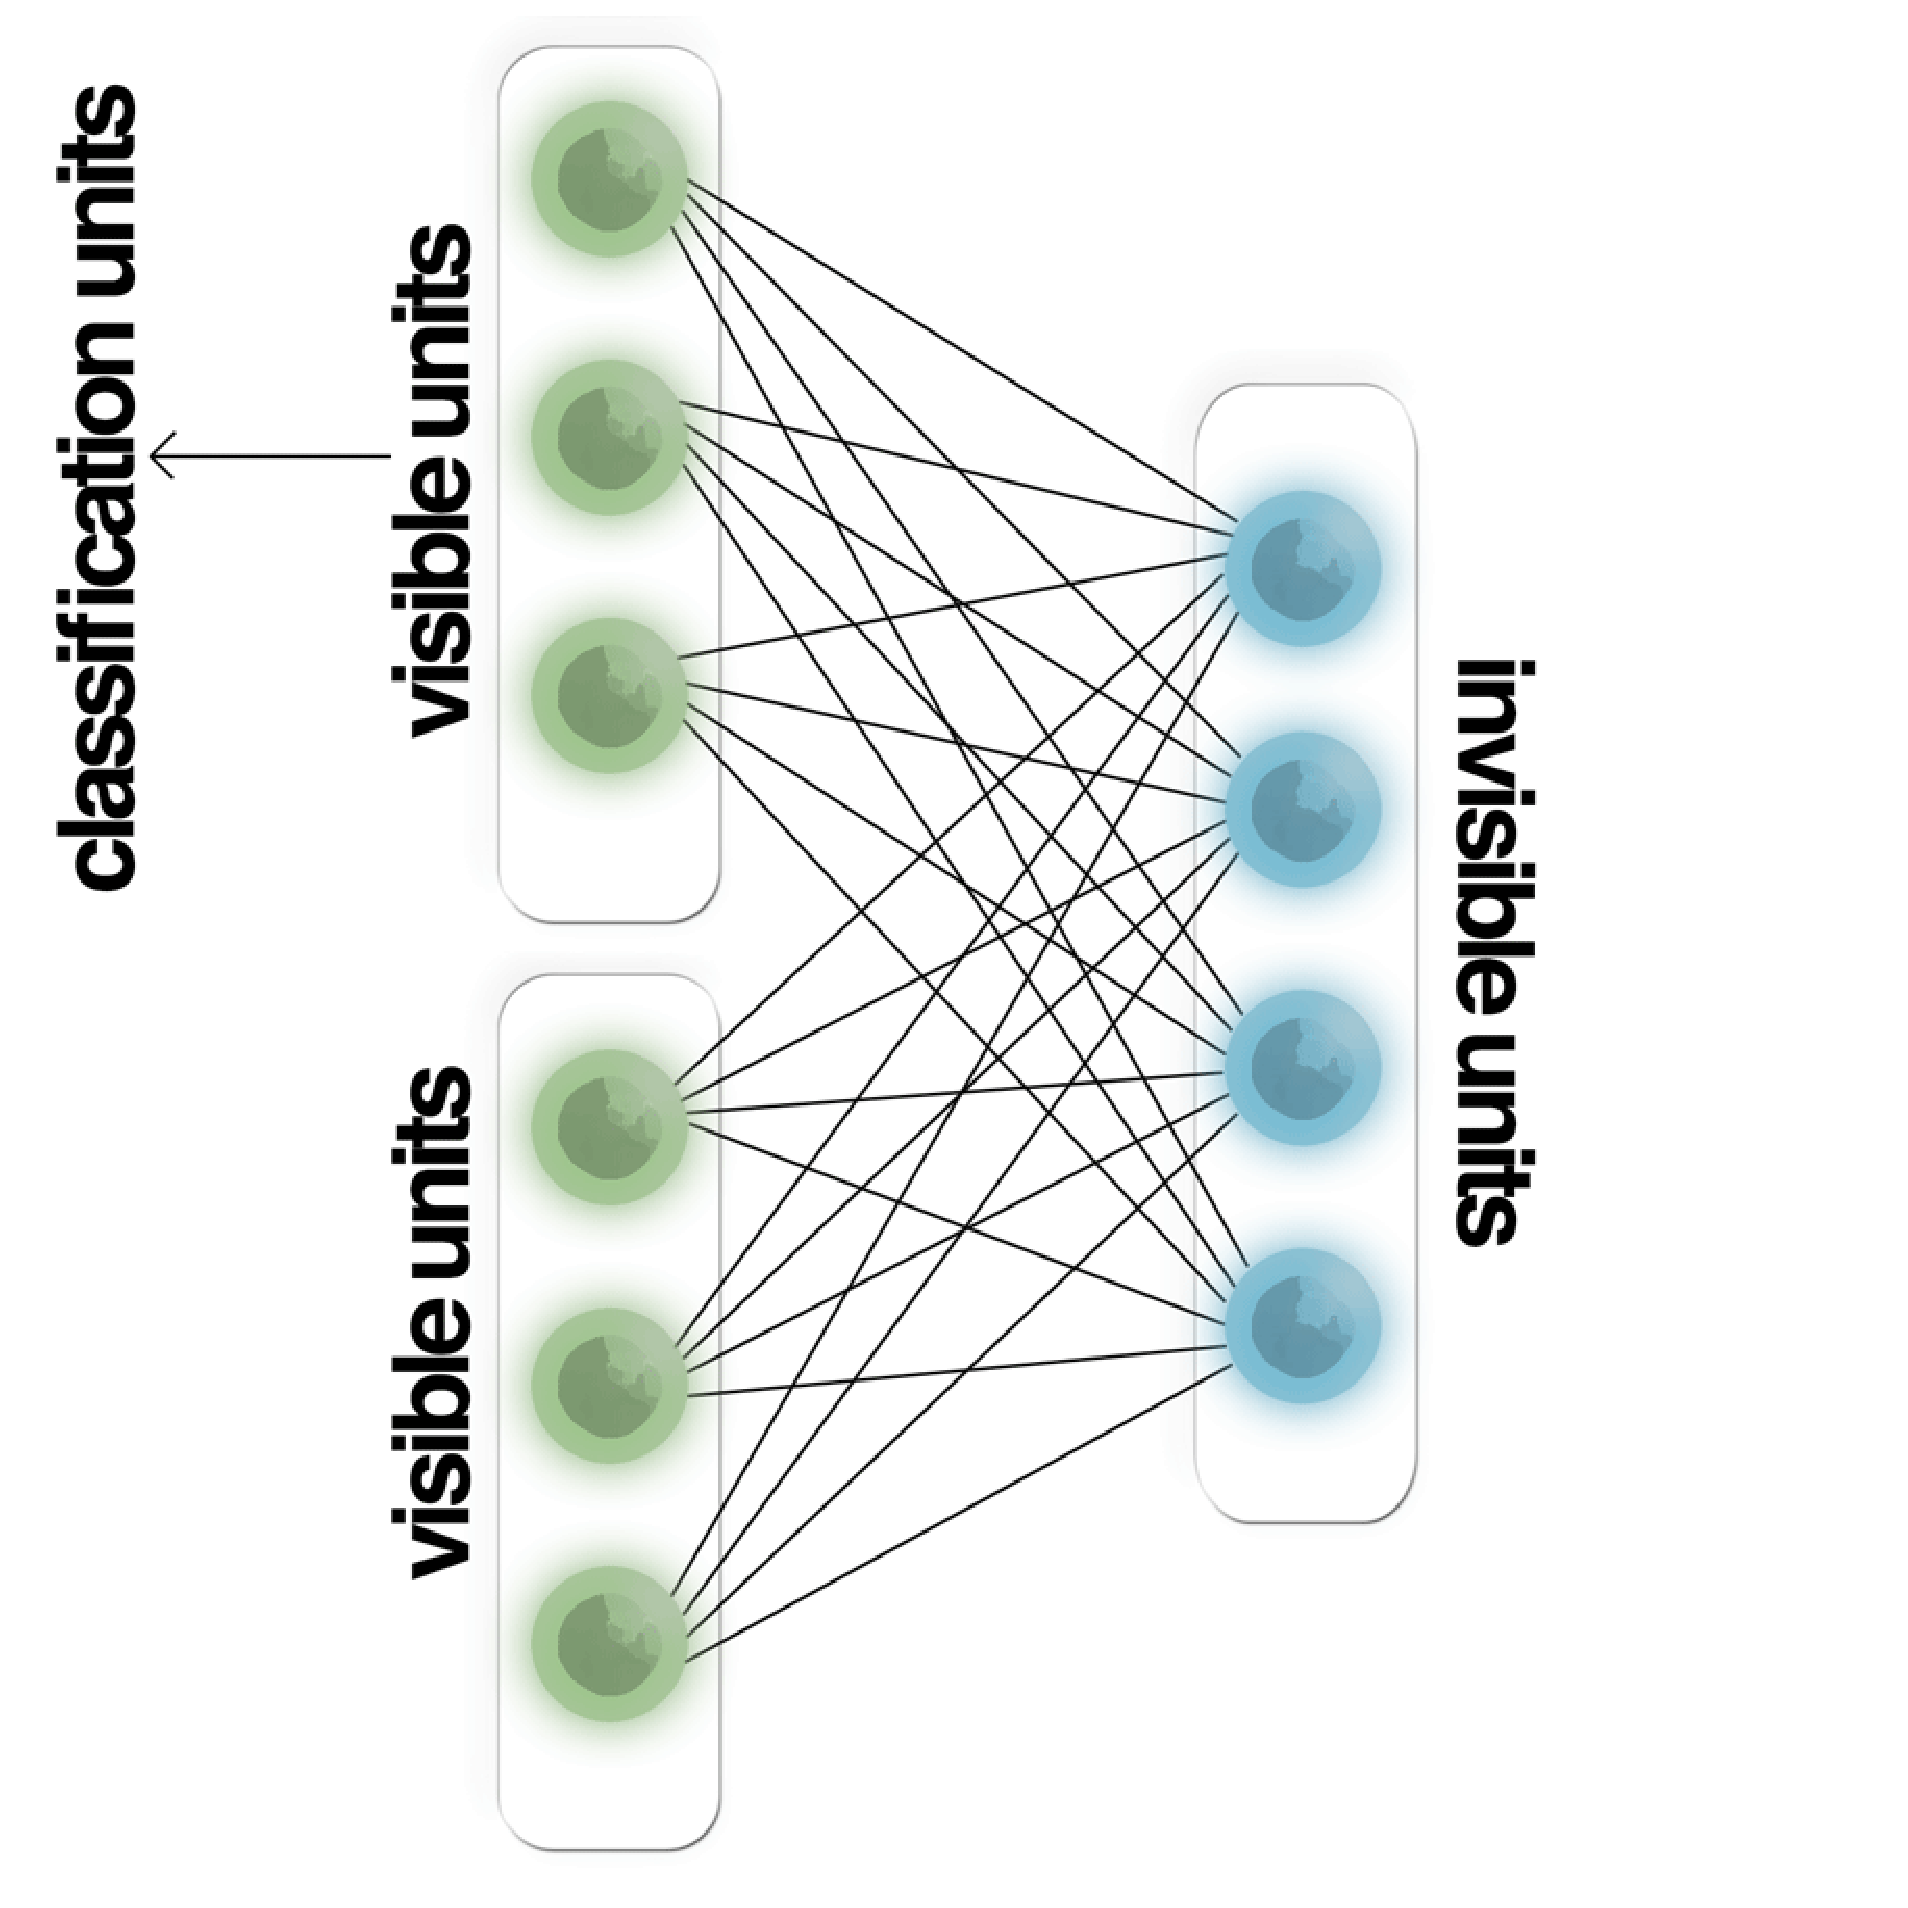
\includegraphics{RBM-2.eps}}
  \caption{Classification Boltzmann machine}
\end{figure}



The vector hidden units is used to model the joint distribution between a
vector of inputs v and a target (classification) vector y. The classification
vector y corresponds to a class. It's length is given by the number of
classes. $y = e_c$, where c is the class the vector is modelling ($e_c$ is a
vector with all zeros, expect from the position c, where it is 1).

As seen from Figure 2, one now needs to weight matrices, which we will denote
by \tmtextit{W}(the weight matrix between the visbile units and hidden ones) \
and U (the weight matrix and between the classification units and hidden
ones). Vectors \tmtextit{b}, \tmtextit{c}, \tmtextit{d} correspond to the
vector of biases for the visible units (training patterns), hidden units and
classification units, respectively.

The energy function for this model is:
\[ E \left( v \nocomma, y, h \right) = - d^T y - c^T h - b^T v - h^T W v - h^T
   U y \]
Which gives rise to the following formula for the probility of a configuration
\tmtextit{v}, \tmtextit{y}.
\[ p \left( v, y, h \right) = \frac{e^{- E \left( v \nocomma, y, h
   \right)}}{Z} \]
where \tmtextit{Z} is the normalizing constant. Thus,
\[ p \left( v, y \right) = \sum_h p \left( v, y, h \right) = \sum_h \frac{e^{-
   E \left( v \nocomma, y, h \right)}}{Z} \]
The distribution used for the Classification Boltzmann Machine are the
following:
\begin{equation}
  p \left( h_i = 1 \left| v, y \right. \right) = \sigma \left( c_j + \noplus
  \noplus W_j v \noplus + U_j y \right)
\end{equation}
\begin{equation}
  p \left( v_i = 1 \left| h \right. \right) = \sigma \left( b_j + \noplus
  \noplus h^T W^i  \right)
\end{equation}
\begin{equation}
  p \left( y = e_c \left| h \right. \right) = \frac{e^{d^T e_c \noplus + h^T
  Ue_c}}{N}
\end{equation}
where N is the normalizing constant $\sum_c$ $e^{d^T e_c \noplus + h^T Ue_c}$.

Note that we denote by $W_i$ the row \tmtextit{i} of matrix \tmtextit{W}, and
by $W^i_{}$ the column \tmtextit{i} of matrix \tmtextit{W}.



Valuable reference for this was given to us from
[http://uai.sis.pitt.edu/papers/11/p463-louradour.pdf and,
http://www.dmi.usherb.ca/\~{ }larocheh/publications/drbm-mitacs-poster.pdf].

\subsection{Learning}

Contrastive divergence can be used to train the network, giving rise to the
following update rules:


\begin{eqnarray*}
  b'  & = & b + \lambda \left( v - v_{\tmop{sampled}} \right)\\
  c'  & = & c + \lambda \left( h_{\sigma} - h_{\sigma \tmop{sampled}}
  \right)\\
  d'  & = & d + \lambda \left( y - y_{\tmop{sampled}} \right)\\
  W'  & = & W + \lambda \left( h_{\sigma} v^T - h_{\sigma \tmop{sampled}}
  v_{\tmop{sampled}}^T \right)\\
  U' & = & U + \lambda \left( \left. h_{\sigma} y^T - h_{\sigma
  \tmop{sampled}} y_{\tmop{sampled}}^T \right) \right.
\end{eqnarray*}
where we denote by $x'$ the new value of parameter x. $v_{\tmop{sampled}} $and
$y_{\tmop{sampled}} $are obtained by sampling the distributions in (5) and
(6).
\begin{eqnarray*}
  h_{\sigma} & = & \sigma \left( c_j + \noplus \noplus W_j v \noplus + U_j y
  \right)\\
  h_{\sigma \tmop{sampled}} & = & \sigma \left( c_j + \noplus \noplus W_j
  v_{\tmop{sampled}} \noplus + U_j y_{\tmop{sampled}}  \right)
\end{eqnarray*}
\subsection{Classification}
\[ p \left( y = e_c \left| v \right. \right) = \frac{e^{- F \left( v \nocomma,
   e_c \right)}}{\sum_d e^{- F \left( v \nocomma, e_d \right)}} \]
where $F \left( v \nocomma, e_c \right) $is the \tmtextit{free energy
function}
\[ F \left( v \nocomma, e_c \right) = - d^T y - \sum^H_{j = 1}
   \tmtextit{\tmtextit{s}} \left( c_j + \noplus \noplus W_j v \noplus + U_j y
   \right) \nocomma \]
where $s \left( x \right) = \log \left( 1 + e^x \right) $



The implementation of the Classification Boltzmann Machine can be found in

\tmtexttt{ClassficationBoltzmannMachine.hs. }



\subsection{New method}

Another method we have employed using Boltzmann Machines was created by us. We
have never seen this approach used somewhere else. Instead of creating 2 types
of visible units, we use the simple Restricted Boltzmann Machine, with one
type of visible units (and hence one single matrix). For each training vector
we append the classification at the end. The classification is represented as
a binary vector, either as above, by using $e_c$, where c is the
classification of the current pattern, or even in a more compressed manner, by
creating the binary vector using the representation in base 2 of class c.

\ \ \ \ \ \ \ \ \ \ \ \ \ \ \ \ \ \ \ \ \ \ \ \ \ \ \ \ \ \ \ \ \ \ \ \ \ \
\ \ \

\ \ \ \ \ \ \ \ \ \ \ \ \ \ \ \ \ \ \ \ \ \ \ \ \ \ \ \ \ \ \ \ \ \ \ \ \

\ \ \ \ \ \ \ \ \ \ \ \ \ \ \ \ \ \begin{figure}[h]
  \ \ \ \ \ \ \ \ \ \ \ \ \
  \resizebox{350px}{350px}{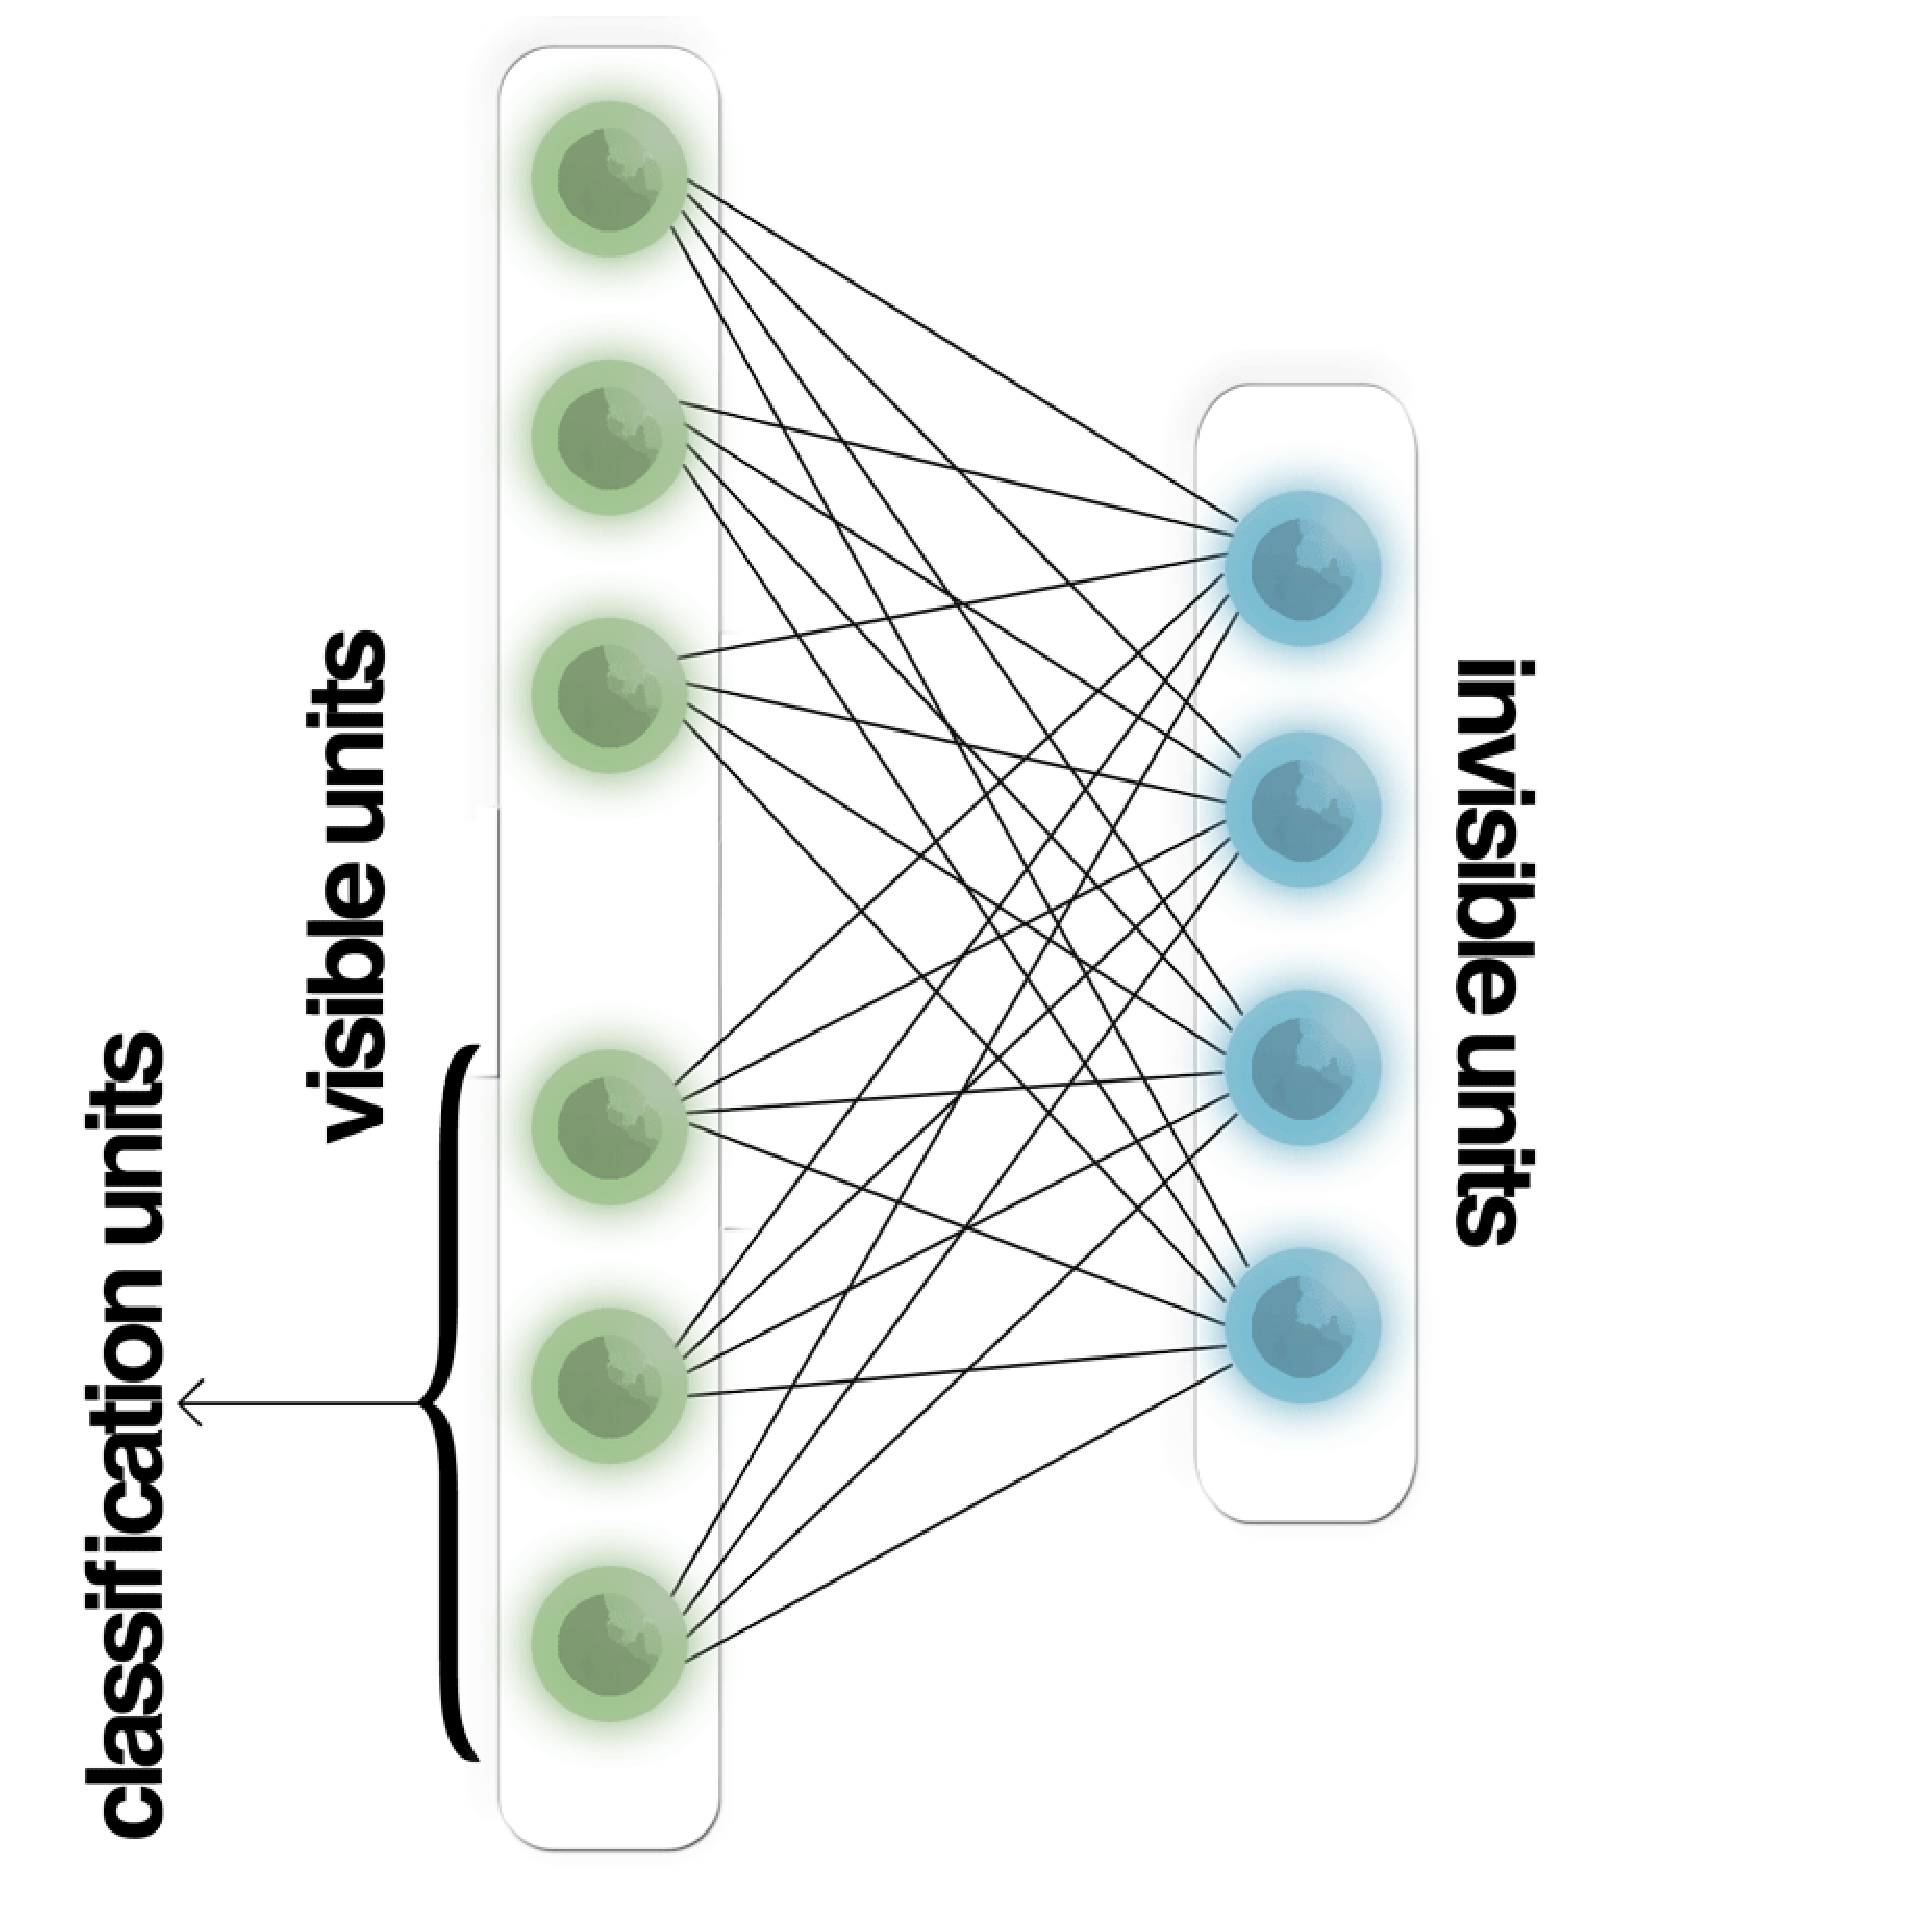
\includegraphics{RBM-3.eps}}
  \caption{Boltzmann machines according to our new method}
\end{figure} \ \ \ \ \ \ \ \ \ \ \ \ \ \ \ \ \ \ \ \ \ \ \ \ \ \ \ \ \ \ \ \ \
\ \ \ \ \ \

\ \ \ \ \ \ \ \ \ \ \ \ \ \ \ \ \ \ \ \ \ \ \ \ \ \ \ \ \ \ \ \ \ \

The training is done in the usual way, but with the complete vectors (actual
pattern and classification). In our case, as different patterns ought to have
different classifcations, we use as class the index of the pattern in the list
(with removed duplicates) of training patterns.

When a pattern needs to be matched to one of the training patterns for
recognition, one uses the log probability (given using ...) to compute the
probability of each of the classifications, and choses the one with maximum
probability.



\begin{figure}[h]
  \resizebox{622px}{182px}{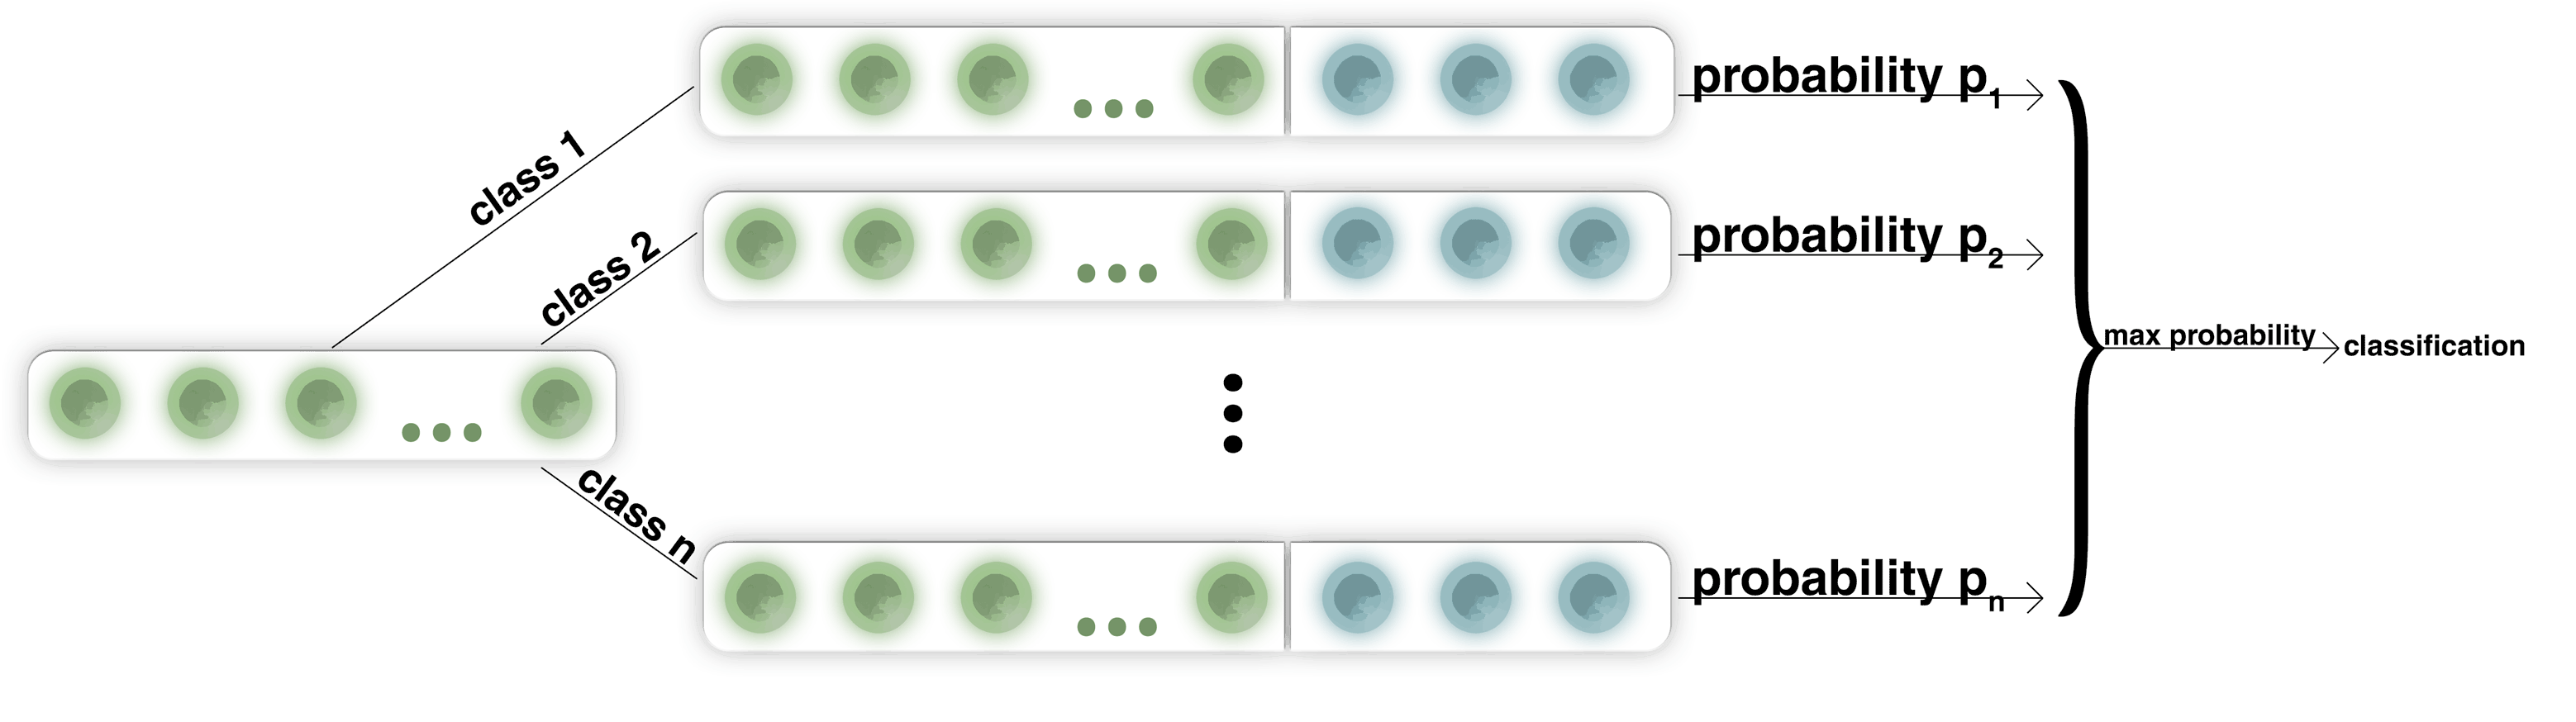
\includegraphics{RBM-4.eps}}
  \caption{The recognition process in the new Boltzmann machine.}
\end{figure}



As given in http://www.cs.toronto.edu/\~{ }hinton/absps/guideTR.pdf, the log
probability is given by:
\[ \tmtextit{\log} \left( \tmop{class} = c \left| v \right. \right) =
   \frac{e^{- F_c \left( v \right)}}{\sum_{c'} e^{- F_{c'} \left( v
   \right)}} \]
\[ F \left( v \right) = - \sum_{i \in V} v_i a_i - \sum_{j \in H} \log \left(
   1 \noplus + e^{x_j} \right) \]


where $x_j = b_j + \sum_i w_{ij_{}} v_j$



The implementation of this procedure can be found in
\tmtexttt{RestrictedBoltzmannMachine.hs.}

